\documentclass{article} % For LaTeX2e
\usepackage{iclr2019_conference,times}

% Optional math commands from https://github.com/goodfeli/dlbook_notation.
%%%%% NEW MATH DEFINITIONS %%%%%

\usepackage{amsmath,amsfonts,bm}

% Mark sections of captions for referring to divisions of figures
\newcommand{\figleft}{{\em (Left)}}
\newcommand{\figcenter}{{\em (Center)}}
\newcommand{\figright}{{\em (Right)}}
\newcommand{\figtop}{{\em (Top)}}
\newcommand{\figbottom}{{\em (Bottom)}}
\newcommand{\captiona}{{\em (a)}}
\newcommand{\captionb}{{\em (b)}}
\newcommand{\captionc}{{\em (c)}}
\newcommand{\captiond}{{\em (d)}}

% Highlight a newly defined term
\newcommand{\newterm}[1]{{\bf #1}}


% Figure reference, lower-case.
\def\figref#1{figure~\ref{#1}}
% Figure reference, capital. For start of sentence
\def\Figref#1{Figure~\ref{#1}}
\def\twofigref#1#2{figures \ref{#1} and \ref{#2}}
\def\quadfigref#1#2#3#4{figures \ref{#1}, \ref{#2}, \ref{#3} and \ref{#4}}
% Section reference, lower-case.
\def\secref#1{section~\ref{#1}}
% Section reference, capital.
\def\Secref#1{Section~\ref{#1}}
% Reference to two sections.
\def\twosecrefs#1#2{sections \ref{#1} and \ref{#2}}
% Reference to three sections.
\def\secrefs#1#2#3{sections \ref{#1}, \ref{#2} and \ref{#3}}
% Reference to an equation, lower-case.
\def\eqref#1{equation~\ref{#1}}
% Reference to an equation, upper case
\def\Eqref#1{Equation~\ref{#1}}
% A raw reference to an equation---avoid using if possible
\def\plaineqref#1{\ref{#1}}
% Reference to a chapter, lower-case.
\def\chapref#1{chapter~\ref{#1}}
% Reference to an equation, upper case.
\def\Chapref#1{Chapter~\ref{#1}}
% Reference to a range of chapters
\def\rangechapref#1#2{chapters\ref{#1}--\ref{#2}}
% Reference to an algorithm, lower-case.
\def\algref#1{algorithm~\ref{#1}}
% Reference to an algorithm, upper case.
\def\Algref#1{Algorithm~\ref{#1}}
\def\twoalgref#1#2{algorithms \ref{#1} and \ref{#2}}
\def\Twoalgref#1#2{Algorithms \ref{#1} and \ref{#2}}
% Reference to a part, lower case
\def\partref#1{part~\ref{#1}}
% Reference to a part, upper case
\def\Partref#1{Part~\ref{#1}}
\def\twopartref#1#2{parts \ref{#1} and \ref{#2}}

\def\ceil#1{\lceil #1 \rceil}
\def\floor#1{\lfloor #1 \rfloor}
\def\1{\bm{1}}
\newcommand{\train}{\mathcal{D}}
\newcommand{\valid}{\mathcal{D_{\mathrm{valid}}}}
\newcommand{\test}{\mathcal{D_{\mathrm{test}}}}

\def\eps{{\epsilon}}


% Random variables
\def\reta{{\textnormal{$\eta$}}}
\def\ra{{\textnormal{a}}}
\def\rb{{\textnormal{b}}}
\def\rc{{\textnormal{c}}}
\def\rd{{\textnormal{d}}}
\def\re{{\textnormal{e}}}
\def\rf{{\textnormal{f}}}
\def\rg{{\textnormal{g}}}
\def\rh{{\textnormal{h}}}
\def\ri{{\textnormal{i}}}
\def\rj{{\textnormal{j}}}
\def\rk{{\textnormal{k}}}
\def\rl{{\textnormal{l}}}
% rm is already a command, just don't name any random variables m
\def\rn{{\textnormal{n}}}
\def\ro{{\textnormal{o}}}
\def\rp{{\textnormal{p}}}
\def\rq{{\textnormal{q}}}
\def\rr{{\textnormal{r}}}
\def\rs{{\textnormal{s}}}
\def\rt{{\textnormal{t}}}
\def\ru{{\textnormal{u}}}
\def\rv{{\textnormal{v}}}
\def\rw{{\textnormal{w}}}
\def\rx{{\textnormal{x}}}
\def\ry{{\textnormal{y}}}
\def\rz{{\textnormal{z}}}

% Random vectors
\def\rvepsilon{{\mathbf{\epsilon}}}
\def\rvtheta{{\mathbf{\theta}}}
\def\rva{{\mathbf{a}}}
\def\rvb{{\mathbf{b}}}
\def\rvc{{\mathbf{c}}}
\def\rvd{{\mathbf{d}}}
\def\rve{{\mathbf{e}}}
\def\rvf{{\mathbf{f}}}
\def\rvg{{\mathbf{g}}}
\def\rvh{{\mathbf{h}}}
\def\rvu{{\mathbf{i}}}
\def\rvj{{\mathbf{j}}}
\def\rvk{{\mathbf{k}}}
\def\rvl{{\mathbf{l}}}
\def\rvm{{\mathbf{m}}}
\def\rvn{{\mathbf{n}}}
\def\rvo{{\mathbf{o}}}
\def\rvp{{\mathbf{p}}}
\def\rvq{{\mathbf{q}}}
\def\rvr{{\mathbf{r}}}
\def\rvs{{\mathbf{s}}}
\def\rvt{{\mathbf{t}}}
\def\rvu{{\mathbf{u}}}
\def\rvv{{\mathbf{v}}}
\def\rvw{{\mathbf{w}}}
\def\rvx{{\mathbf{x}}}
\def\rvy{{\mathbf{y}}}
\def\rvz{{\mathbf{z}}}

% Elements of random vectors
\def\erva{{\textnormal{a}}}
\def\ervb{{\textnormal{b}}}
\def\ervc{{\textnormal{c}}}
\def\ervd{{\textnormal{d}}}
\def\erve{{\textnormal{e}}}
\def\ervf{{\textnormal{f}}}
\def\ervg{{\textnormal{g}}}
\def\ervh{{\textnormal{h}}}
\def\ervi{{\textnormal{i}}}
\def\ervj{{\textnormal{j}}}
\def\ervk{{\textnormal{k}}}
\def\ervl{{\textnormal{l}}}
\def\ervm{{\textnormal{m}}}
\def\ervn{{\textnormal{n}}}
\def\ervo{{\textnormal{o}}}
\def\ervp{{\textnormal{p}}}
\def\ervq{{\textnormal{q}}}
\def\ervr{{\textnormal{r}}}
\def\ervs{{\textnormal{s}}}
\def\ervt{{\textnormal{t}}}
\def\ervu{{\textnormal{u}}}
\def\ervv{{\textnormal{v}}}
\def\ervw{{\textnormal{w}}}
\def\ervx{{\textnormal{x}}}
\def\ervy{{\textnormal{y}}}
\def\ervz{{\textnormal{z}}}

% Random matrices
\def\rmA{{\mathbf{A}}}
\def\rmB{{\mathbf{B}}}
\def\rmC{{\mathbf{C}}}
\def\rmD{{\mathbf{D}}}
\def\rmE{{\mathbf{E}}}
\def\rmF{{\mathbf{F}}}
\def\rmG{{\mathbf{G}}}
\def\rmH{{\mathbf{H}}}
\def\rmI{{\mathbf{I}}}
\def\rmJ{{\mathbf{J}}}
\def\rmK{{\mathbf{K}}}
\def\rmL{{\mathbf{L}}}
\def\rmM{{\mathbf{M}}}
\def\rmN{{\mathbf{N}}}
\def\rmO{{\mathbf{O}}}
\def\rmP{{\mathbf{P}}}
\def\rmQ{{\mathbf{Q}}}
\def\rmR{{\mathbf{R}}}
\def\rmS{{\mathbf{S}}}
\def\rmT{{\mathbf{T}}}
\def\rmU{{\mathbf{U}}}
\def\rmV{{\mathbf{V}}}
\def\rmW{{\mathbf{W}}}
\def\rmX{{\mathbf{X}}}
\def\rmY{{\mathbf{Y}}}
\def\rmZ{{\mathbf{Z}}}

% Elements of random matrices
\def\ermA{{\textnormal{A}}}
\def\ermB{{\textnormal{B}}}
\def\ermC{{\textnormal{C}}}
\def\ermD{{\textnormal{D}}}
\def\ermE{{\textnormal{E}}}
\def\ermF{{\textnormal{F}}}
\def\ermG{{\textnormal{G}}}
\def\ermH{{\textnormal{H}}}
\def\ermI{{\textnormal{I}}}
\def\ermJ{{\textnormal{J}}}
\def\ermK{{\textnormal{K}}}
\def\ermL{{\textnormal{L}}}
\def\ermM{{\textnormal{M}}}
\def\ermN{{\textnormal{N}}}
\def\ermO{{\textnormal{O}}}
\def\ermP{{\textnormal{P}}}
\def\ermQ{{\textnormal{Q}}}
\def\ermR{{\textnormal{R}}}
\def\ermS{{\textnormal{S}}}
\def\ermT{{\textnormal{T}}}
\def\ermU{{\textnormal{U}}}
\def\ermV{{\textnormal{V}}}
\def\ermW{{\textnormal{W}}}
\def\ermX{{\textnormal{X}}}
\def\ermY{{\textnormal{Y}}}
\def\ermZ{{\textnormal{Z}}}

% Vectors
\def\vzero{{\bm{0}}}
\def\vone{{\bm{1}}}
\def\vmu{{\bm{\mu}}}
\def\vtheta{{\bm{\theta}}}
\def\va{{\bm{a}}}
\def\vb{{\bm{b}}}
\def\vc{{\bm{c}}}
\def\vd{{\bm{d}}}
\def\ve{{\bm{e}}}
\def\vf{{\bm{f}}}
\def\vg{{\bm{g}}}
\def\vh{{\bm{h}}}
\def\vi{{\bm{i}}}
\def\vj{{\bm{j}}}
\def\vk{{\bm{k}}}
\def\vl{{\bm{l}}}
\def\vm{{\bm{m}}}
\def\vn{{\bm{n}}}
\def\vo{{\bm{o}}}
\def\vp{{\bm{p}}}
\def\vq{{\bm{q}}}
\def\vr{{\bm{r}}}
\def\vs{{\bm{s}}}
\def\vt{{\bm{t}}}
\def\vu{{\bm{u}}}
\def\vv{{\bm{v}}}
\def\vw{{\bm{w}}}
\def\vx{{\bm{x}}}
\def\vy{{\bm{y}}}
\def\vz{{\bm{z}}}

% Elements of vectors
\def\evalpha{{\alpha}}
\def\evbeta{{\beta}}
\def\evepsilon{{\epsilon}}
\def\evlambda{{\lambda}}
\def\evomega{{\omega}}
\def\evmu{{\mu}}
\def\evpsi{{\psi}}
\def\evsigma{{\sigma}}
\def\evtheta{{\theta}}
\def\eva{{a}}
\def\evb{{b}}
\def\evc{{c}}
\def\evd{{d}}
\def\eve{{e}}
\def\evf{{f}}
\def\evg{{g}}
\def\evh{{h}}
\def\evi{{i}}
\def\evj{{j}}
\def\evk{{k}}
\def\evl{{l}}
\def\evm{{m}}
\def\evn{{n}}
\def\evo{{o}}
\def\evp{{p}}
\def\evq{{q}}
\def\evr{{r}}
\def\evs{{s}}
\def\evt{{t}}
\def\evu{{u}}
\def\evv{{v}}
\def\evw{{w}}
\def\evx{{x}}
\def\evy{{y}}
\def\evz{{z}}

% Matrix
\def\mA{{\bm{A}}}
\def\mB{{\bm{B}}}
\def\mC{{\bm{C}}}
\def\mD{{\bm{D}}}
\def\mE{{\bm{E}}}
\def\mF{{\bm{F}}}
\def\mG{{\bm{G}}}
\def\mH{{\bm{H}}}
\def\mI{{\bm{I}}}
\def\mJ{{\bm{J}}}
\def\mK{{\bm{K}}}
\def\mL{{\bm{L}}}
\def\mM{{\bm{M}}}
\def\mN{{\bm{N}}}
\def\mO{{\bm{O}}}
\def\mP{{\bm{P}}}
\def\mQ{{\bm{Q}}}
\def\mR{{\bm{R}}}
\def\mS{{\bm{S}}}
\def\mT{{\bm{T}}}
\def\mU{{\bm{U}}}
\def\mV{{\bm{V}}}
\def\mW{{\bm{W}}}
\def\mX{{\bm{X}}}
\def\mY{{\bm{Y}}}
\def\mZ{{\bm{Z}}}
\def\mBeta{{\bm{\beta}}}
\def\mPhi{{\bm{\Phi}}}
\def\mLambda{{\bm{\Lambda}}}
\def\mSigma{{\bm{\Sigma}}}

% Tensor
\DeclareMathAlphabet{\mathsfit}{\encodingdefault}{\sfdefault}{m}{sl}
\SetMathAlphabet{\mathsfit}{bold}{\encodingdefault}{\sfdefault}{bx}{n}
\newcommand{\tens}[1]{\bm{\mathsfit{#1}}}
\def\tA{{\tens{A}}}
\def\tB{{\tens{B}}}
\def\tC{{\tens{C}}}
\def\tD{{\tens{D}}}
\def\tE{{\tens{E}}}
\def\tF{{\tens{F}}}
\def\tG{{\tens{G}}}
\def\tH{{\tens{H}}}
\def\tI{{\tens{I}}}
\def\tJ{{\tens{J}}}
\def\tK{{\tens{K}}}
\def\tL{{\tens{L}}}
\def\tM{{\tens{M}}}
\def\tN{{\tens{N}}}
\def\tO{{\tens{O}}}
\def\tP{{\tens{P}}}
\def\tQ{{\tens{Q}}}
\def\tR{{\tens{R}}}
\def\tS{{\tens{S}}}
\def\tT{{\tens{T}}}
\def\tU{{\tens{U}}}
\def\tV{{\tens{V}}}
\def\tW{{\tens{W}}}
\def\tX{{\tens{X}}}
\def\tY{{\tens{Y}}}
\def\tZ{{\tens{Z}}}


% Graph
\def\gA{{\mathcal{A}}}
\def\gB{{\mathcal{B}}}
\def\gC{{\mathcal{C}}}
\def\gD{{\mathcal{D}}}
\def\gE{{\mathcal{E}}}
\def\gF{{\mathcal{F}}}
\def\gG{{\mathcal{G}}}
\def\gH{{\mathcal{H}}}
\def\gI{{\mathcal{I}}}
\def\gJ{{\mathcal{J}}}
\def\gK{{\mathcal{K}}}
\def\gL{{\mathcal{L}}}
\def\gM{{\mathcal{M}}}
\def\gN{{\mathcal{N}}}
\def\gO{{\mathcal{O}}}
\def\gP{{\mathcal{P}}}
\def\gQ{{\mathcal{Q}}}
\def\gR{{\mathcal{R}}}
\def\gS{{\mathcal{S}}}
\def\gT{{\mathcal{T}}}
\def\gU{{\mathcal{U}}}
\def\gV{{\mathcal{V}}}
\def\gW{{\mathcal{W}}}
\def\gX{{\mathcal{X}}}
\def\gY{{\mathcal{Y}}}
\def\gZ{{\mathcal{Z}}}

% Sets
\def\sA{{\mathbb{A}}}
\def\sB{{\mathbb{B}}}
\def\sC{{\mathbb{C}}}
\def\sD{{\mathbb{D}}}
% Don't use a set called E, because this would be the same as our symbol
% for expectation.
\def\sF{{\mathbb{F}}}
\def\sG{{\mathbb{G}}}
\def\sH{{\mathbb{H}}}
\def\sI{{\mathbb{I}}}
\def\sJ{{\mathbb{J}}}
\def\sK{{\mathbb{K}}}
\def\sL{{\mathbb{L}}}
\def\sM{{\mathbb{M}}}
\def\sN{{\mathbb{N}}}
\def\sO{{\mathbb{O}}}
\def\sP{{\mathbb{P}}}
\def\sQ{{\mathbb{Q}}}
\def\sR{{\mathbb{R}}}
\def\sS{{\mathbb{S}}}
\def\sT{{\mathbb{T}}}
\def\sU{{\mathbb{U}}}
\def\sV{{\mathbb{V}}}
\def\sW{{\mathbb{W}}}
\def\sX{{\mathbb{X}}}
\def\sY{{\mathbb{Y}}}
\def\sZ{{\mathbb{Z}}}

% Entries of a matrix
\def\emLambda{{\Lambda}}
\def\emA{{A}}
\def\emB{{B}}
\def\emC{{C}}
\def\emD{{D}}
\def\emE{{E}}
\def\emF{{F}}
\def\emG{{G}}
\def\emH{{H}}
\def\emI{{I}}
\def\emJ{{J}}
\def\emK{{K}}
\def\emL{{L}}
\def\emM{{M}}
\def\emN{{N}}
\def\emO{{O}}
\def\emP{{P}}
\def\emQ{{Q}}
\def\emR{{R}}
\def\emS{{S}}
\def\emT{{T}}
\def\emU{{U}}
\def\emV{{V}}
\def\emW{{W}}
\def\emX{{X}}
\def\emY{{Y}}
\def\emZ{{Z}}
\def\emSigma{{\Sigma}}

% entries of a tensor
% Same font as tensor, without \bm wrapper
\newcommand{\etens}[1]{\mathsfit{#1}}
\def\etLambda{{\etens{\Lambda}}}
\def\etA{{\etens{A}}}
\def\etB{{\etens{B}}}
\def\etC{{\etens{C}}}
\def\etD{{\etens{D}}}
\def\etE{{\etens{E}}}
\def\etF{{\etens{F}}}
\def\etG{{\etens{G}}}
\def\etH{{\etens{H}}}
\def\etI{{\etens{I}}}
\def\etJ{{\etens{J}}}
\def\etK{{\etens{K}}}
\def\etL{{\etens{L}}}
\def\etM{{\etens{M}}}
\def\etN{{\etens{N}}}
\def\etO{{\etens{O}}}
\def\etP{{\etens{P}}}
\def\etQ{{\etens{Q}}}
\def\etR{{\etens{R}}}
\def\etS{{\etens{S}}}
\def\etT{{\etens{T}}}
\def\etU{{\etens{U}}}
\def\etV{{\etens{V}}}
\def\etW{{\etens{W}}}
\def\etX{{\etens{X}}}
\def\etY{{\etens{Y}}}
\def\etZ{{\etens{Z}}}

% The true underlying data generating distribution
\newcommand{\pdata}{p_{\rm{data}}}
% The empirical distribution defined by the training set
\newcommand{\ptrain}{\hat{p}_{\rm{data}}}
\newcommand{\Ptrain}{\hat{P}_{\rm{data}}}
% The model distribution
\newcommand{\pmodel}{p_{\rm{model}}}
\newcommand{\Pmodel}{P_{\rm{model}}}
\newcommand{\ptildemodel}{\tilde{p}_{\rm{model}}}
% Stochastic autoencoder distributions
\newcommand{\pencode}{p_{\rm{encoder}}}
\newcommand{\pdecode}{p_{\rm{decoder}}}
\newcommand{\precons}{p_{\rm{reconstruct}}}

\newcommand{\laplace}{\mathrm{Laplace}} % Laplace distribution

\newcommand{\E}{\mathbb{E}}
\newcommand{\Ls}{\mathcal{L}}
\newcommand{\R}{\mathbb{R}}
\newcommand{\emp}{\tilde{p}}
\newcommand{\lr}{\alpha}
\newcommand{\reg}{\lambda}
\newcommand{\rect}{\mathrm{rectifier}}
\newcommand{\softmax}{\mathrm{softmax}}
\newcommand{\sigmoid}{\sigma}
\newcommand{\softplus}{\zeta}
\newcommand{\KL}{D_{\mathrm{KL}}}
\newcommand{\Var}{\mathrm{Var}}
\newcommand{\standarderror}{\mathrm{SE}}
\newcommand{\Cov}{\mathrm{Cov}}
% Wolfram Mathworld says $L^2$ is for function spaces and $\ell^2$ is for vectors
% But then they seem to use $L^2$ for vectors throughout the site, and so does
% wikipedia.
\newcommand{\normlzero}{L^0}
\newcommand{\normlone}{L^1}
\newcommand{\normltwo}{L^2}
\newcommand{\normlp}{L^p}
\newcommand{\normmax}{L^\infty}

\newcommand{\parents}{Pa} % See usage in notation.tex. Chosen to match Daphne's book.

\DeclareMathOperator*{\argmax}{arg\,max}
\DeclareMathOperator*{\argmin}{arg\,min}

\DeclareMathOperator{\sign}{sign}
\DeclareMathOperator{\Tr}{Tr}
\let\ab\allowbreak


% More commands
\newcommand{\reminder}[1]{{\color{red}#1}}
\newcommand{\spara}[1]{\smallskip\noindent{\bf #1}}
\newcommand{\mpara}[1]{\medskip\noindent{\bf #1}}
\newcommand{\para}[1]{\noindent{\bf #1}}


\usepackage{hyperref}
\usepackage{url}
\usepackage{graphicx}
\usepackage{booktabs}
\usepackage{multirow}
\usepackage{caption}
\usepackage{colortbl}

\graphicspath{{./figures/}}

\title{A Comparative Evaluation on Network \\Representation Learning Techniques}

% Authors must not appear in the submitted version. They should be hidden
% as long as the \iclrfinalcopy macro remains commented out below.
% Non-anonymous submissions will be rejected without review.

\author{Konstantinos Ameranis \And Panagiota Kiourti \And Konstantinos Sotiropoulos \AND Erasmo Tani \And Isidora Tourni}

% The \author macro works with any number of authors. There are two commands
% used to separate the names and addresses of multiple authors: \And and \AND.
%
% Using \And between authors leaves it to \LaTeX{} to determine where to break
% the lines. Using \AND forces a linebreak at that point. So, if \LaTeX{}
% puts 3 of 4 authors names on the first line, and the last on the second
% line, try using \AND instead of \And before the third author name.

\newcommand{\fix}{\marginpar{FIX}}
\newcommand{\new}{\marginpar{NEW}}

\iclrfinalcopy % Uncomment for camera-ready version, but NOT for submission.
\begin{document}


\maketitle

\begin{abstract}
The abstract paragraph should be indented 1/2~inch (3~picas) on both left and
right-hand margins. Use 10~point type, with a vertical spacing of 11~points.
The word \textsc{Abstract} must be centered, in small caps, and in point size 12. Two
line spaces precede the abstract. The abstract must be limited to one
paragraph.
\end{abstract}

\section{Introduction}
Graph data is pervasive in modern data analysis. In Computer Science, graphs have been an object of study for decades, representing a fundamental tool in the area of data structures and algorithms, and a model for systems ranging from computer networks and social networks to the World Wide Web. The impact of graphs has however vastly exceeded the boundaries of Computer Science, as these models have been used in fields as diverse as Biology, where they represent, for instance protein interaction networks, and Operation Research, in which they appear as models infrastructure networks, such as systems of roads or pipes.

In order to analyze network data it is often useful to obtain a representation of the vertices of the graph in Euclidean Space (an \textbf{embedding}). This allows us to leverage the power of machine learning and data mining techniques that are tailored to Euclidean setting and use them to make sense of the properties of the graph. In order for this to work, the embedding has to somehow encode some of the information and patterns that were contained in the original network. Some desirable properties the embedding should satisfy are the following (\cite{chen2018tutorial}):

\textbf{1. Adaptability} Since data might be changing over time, the embedding should be efficiently updatable,\\
\textbf{2. Scalability} The embedding should be computable on large graphs,\\
\textbf{3. Community Awareness} The Euclidean distance in the embedding should reflect the community structure of the underlying graph,\\
\textbf{4. Low Dimensionality} Having a low dimensional embedding often allows for better generalization.\\


The problem of finding the best such embedding has proved to be far from trivial, and while many solutions have been proposed, there appears to be no universal answer.

In this project we will look at some of the embedding techniques that have been developed and test their effectiveness in the context of a simple machine learning task.


\subsection{Definitions}
We now introduce our objects of study.

A \textbf{(undirected) graph} is a pair $(V,E)$, where $V$ is a finite set of \textbf{vertices} (/nodes) and $E$ is a collection of \textbf{edges} (/links). Each element of $E$ is a two-element subset $\{v,u\}$ of $V$, encoding the property that the vertex $v \in V$ is connected to the vertex $u \in V$.\\

A graph \textbf{embedding} for a given graph $G = (V,E)$ is a function $\Phi:V \to \mathbb{R}^{|V| \times d}$.

\section{Network Embeddings}

\subsection{Matrix Factorization}
\subsubsection*{Multidimensional Scaling (MDS)}
Multidimensional Scaling (MDS) (see \cite{cox2000multidimensional} and \cite{borg2003modern}) is a method for creating a Euclidean embedding of data for which one has distance / dissimilarity information. For instance, given an $N \times N$ matrix of distances between $N$ points, one can embed the points into $\mathbb{R}^k$ so as to preserve distance information. In particular, one can use MDS as a way to create useful features for graphs by considering the shortest path distance between vertices. MDS is similar to PCA, except instead of using correlation information, we make use of pointwise distances.

Classical Multidimensional Scaling works as follows: let $D$ be the dissimilarity matrix. Then:
\begin{enumerate}
  \item Let $D^{(2)}$ be the point-wise square of the distance matrix,
  \item Let $J = I - {1\over n}\vec{1}\vec{1}^T$,
  \item Let $B = -{1 \over 2}JD^{(2)}J$,
  \item Find the top $m$ eigenvalues of $B$ $\lambda_1, ... \lambda_m$, and the corresponding eigenvalues $e_1, ... , e_m$,
  \item Let $X = E_m\Lambda^{1/2}$.
\end{enumerate}

Classical Multidimensional Scaling minimizes a loss function called \emph{strain}:
\[
    \text{Strain}_D(x_1, ... , x_N) = \left( ({\sum_{i,j}b_{i,j}- \langle x_i,x_j \rangle})^2 \over \sum_{i,j}b_{i,j}^2\right).
\]

Classical MDS only works for Euclidean spaces, so in the context of graphs, where the underlying metric is given by shortest path metric, we use a slightly different version of MDS. This variant, known as metric MDS, finds en embedding $x_1, ... , x_n$ minimizing the following objective function (stress):
\[
    \text{Stress}_D(x_1, ... , x_n) = \left(\sum_{i \neq j = 1, ... ,N}(d_{ij} - ||x_i - x_j||)^2\right)^{1/2}
\]



\subsubsection*{Spectral Embedding}
Another way to embed a graph in Euclidean space is given by the spectral embedding. This method computes the $k$ eigenvectors of the normalized Laplacian matrix $\mathcal{L}$  corresponding to the $k$ smallest eigenvalues, and uses each of them as an embedding of the  vertices into $\mathbb{R}$, resulting in an  embedding into $\mathbb{R}^k$. The normalized Laplacian matrix is given by:
\[
    \mathcal{L} = D^{-{1\over 2}}(D - A)D^{-{1\over 2}}
\]

Where $D$ is the $n \times n$ diagonal matrix of degrees of vertices and $A$ is the graph adjacency matrix. One can prove that the quadratic form of the Laplacian is a relaxation to the minimum conductance cut problem (see for instance \cite{chung1997spectral}) defined as follows:

\[
    \underset{S  \subseteq V }{\text{minimize}} {|E(S,\overline{S})|\over \min\{vol(S), vol(\overline{S})\}}.
\]
The eigenvectors of the Laplacian therefore act as optimizers of the relaxation, and tend to align points in space so as to keep connected points close to each other. Note that eigenvectors of the normalized Laplacian are solutions to the generalized eigenvalue problem:
\[
    L\mathbf{x} = \lambda D\mathbf{x}
\]
where $L$ is the (non-normalized) Laplacian matrix: $L = D-A$ and $D$ is defined as above. Spectral embeddings based on the Laplacian are common primitives used in other methods, such as manifold learning, (see for instance \cite{belkin2003laplacian}).

\iffalse
\subsubsection*{Isomap}
Isomap is a method for manifold learning / non-linear dimensionality reduction. In a general setting, given data points living in a (non-linear) manifold in $\mathbb{R}^n$ we would like to embed them into lower dimensional space while preserving geodesic distances.
\fi

\subsection{Random Walks}

A \emph{random walk}, a term first introduced in~\cite{pearson1905problem},
is a sequence of elements or a path on a mathematical space
produced by a random process. Among other applications, random walks are used
for sampling large graphs of social networks.
At a high level a random walk in a graph is a sequence of nodes. This sequence
can be thought of as a sentence where each `node' is a `word'. Therefore, this
analogy let us directly use techniques of word embeddings, for obtaining
embeddings of the nodes. In the next two sections, we introduce
two algorithms that use random walks to learn embeddings of the nodes
by applying an approach that was introduced for learning word embeddings.

\subsubsection{Deepwalk}

Deepwalk is an algorithm that takes a graph as an input, and learns a latent
representation of the nodes. This representation is a vector with continuous
values. The goal is for this representation to capture the social similarity
between the nodes and have a low dimension. In order to learn this
representation, deepwalk uses random walks and assumes that these walks can
capture well the similarity between nodes. First it produces random walks by
selecting a node $v_i$ uniformly at random, from the set of nodes $V$, as the
root of the random walk $W_{v_i}$. Then, it samples one node from the set of the
neighbor nodes of $v_i$ uniformly at random. The last step is now repeated for
each new sampled node until the walk reaches a specific length. Having $\gamma$
such random walks, deepwalk adapts the word2vec approach for obtaining word
embeddings, by treating the random walks as sentences, and the nodes as words.

The \emph{word2vec} method, introduced in \cite{mikolov2013efficient}, is a
method for embedding words of a corpus in a subspace $\mathbb{R}^d$ so that
each embeddings of a specific word can be used to predict the context around this
word, i.e. the words within a window $w$ in a sentence. Specifically, we
want to calculate the probability of every word of the vocabulary being
within a window from the current word (Skip-gram method).
In order to do that, skip-gram parses the words of a given corpus and creates
pairs of words $(w_i, w_j)$ that are within a window $w$, in order to specify
that $w_i$ and $w_j$ are within this window, which means that the two words
are in the same context. Therefore, this method assumes that words that are
`close' inside a sentence, correspond to the same context. These pairs
$(w_i, w_j)$ can be then used as a training set, to train a model to predict the
`nearby' words based on the training set with high probability, i.e. maximizing
the likelihood of the training set. The key idea is that the training of this
model proposes an embedding for each word in the $\mathbb{R}^d$.
Using this embedding we can represent each word as a vector with dimension $d$
which captures the context similarity instead of using an one-hot vector of
dimension equal to the size of the vocabulary. The parameter $d$ is set by the
user and it can be tuned using a validation set.
% Explain homofilous

Deepwalk adapts the idea of word embeddings to graphs by treating the nodes as
words and random walks as sentences. Similarly to the language model, the goal
is to capture node similarity which can be then used for classifying them.
There is no justification about why random walks can capture community
similarity information in a social network graph. However, the authors
%that random walks have been used for capturing
%similarities in a variety of problems. They also
observe that word frequency in some corpora, such as the English Wikipedia,
follows a power-law distribution, which is also the case for the degree of nodes
in social networks and that
possibly makes the random walk suitable for capturing the neighborhood
similarity and community membership in the social network graphs.

Deepwalk initializes a mapping
$\Phi: \mathbb{R}^{\mid V \mid \times S} \to \mathbb{R}^{\mid V\mid \times d}$
where $S$ in the size of the features space. Then, using random walks deepwalk
solves the following optimization problem:
\begin{align}
    \min_{\Phi}
        \left (-\log{Pr({v_{i-w},
                \ldots, v_{i-1}, v_{i+1},
                \ldots , v_{i+w}} \mid \Phi(v_i))}
        \right )
\end{align}
where $v_i$ is the node currently examined in the random walk and
$v_{i-w}, \ldots, \ldots, v_{i-1}, v_{i+1},\ldots, v_{i+w}$ are the nodes
within a window $w$ from the node $v_i$ in this walk. The gradient of the above
quantity with respect to $\Phi$ is
computed in order to update the mapping $\Phi$. In the end, deepwalk outputs
the matrix $\Phi$.

\subsubsection{Node2vec}

Similarly to Deepwalk, \emph{Node2vec} (\cite{grover2016node2vec}) is a method
for learning latent representations of the nodes by using random walks and the
skip-gram. However, this method uses a different way of sampling neighbor
nodes during a random walk, in order to handle graphs that have more structural
equivalent nodes different that the ones that include highly interconnected
nodes.

Node2vec introduces two baselines cases for sampling neighbor nodes: the
Breadth-first Sampling (BFS) and the Depth-first Sampling (DFS).
The Breadth-first strategy samples a neighborhood for a node $v_i$ by
considering as neighbors, the nodes that have an immediate edge to $v_i$.
In contrast, Depth-first strategy considers as neighbors the nodes that are
one more edge away from $v_i$ each time a neighborhood needed should include
more than one node. As an example, consider the node $u$ in
Fig~\ref{sampling_strategies} (obtained by the original
paper~\cite{grover2016node2vec}). Sampling a neighborhood of size 3 using the
BFS strategy can give us the nodes $s_1, s_2, s_3$, while using the DFS strategy
can give us the nodes $s_4, s_5, s_6$.
\begin{figure}
\begin{center}
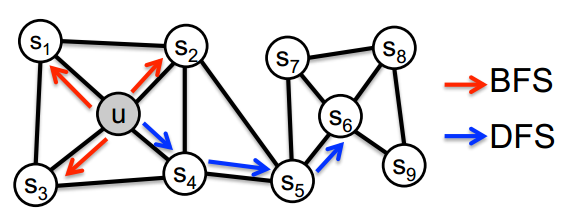
\includegraphics[width=0.7\textwidth]{figures/sampling.png}
\end{center}
\caption{Using the BFS sampling strategy, we can obtain the nodes
$s_1, s_2, s_3$ as the 3 neighbors of $u$. Using the DFS sampling strategy we
can obtain $\{s_4, s_5, s_6\}$. The figure is copied from the original
paper~\cite{grover2016node2vec}.}
\label{sampling_strategies}
\end{figure}
The BFS strategy can create random walks that capture the structural similarities
between nodes. For example, consider a network graphs with nodes that correspond
to hubs or bridges. In this case the embedding will reflect the structural
equivalence of the nodes of the graph.
On the contrary, the DFS strategy samples nodes in a way that explores
neighborhoods of nodes that exhibit \emph{homophily}, which means that nodes
highly connected belong to similar clusters/communities.

Real-world graph networks can be thought of as a mixture of networks that
include structural similar nodes and the ones networks that include nodes which
exhibit homophily. The node2vec approach tries to capture these similarities each
time based on the graph by introducing the parameters $p$, $q$. The return parameter $p$ controls the
likelihood of visiting the node already visited before the current node, or in
other words the likelihood of returning back to the node from which a node was
sampled as a neighbor. The parameter $q$ controls the decision between a BFS and
a DFS sampling strategy. If $q$ is less than 1 then the walk is more biased
to choose nodes that are further from the current node in the walk, while if $q$
is more than 1, then the walk would choose nodes that are close to the current
node with higher probability. Formally, the walk samples using the transition
probabilities $\pi_{ux}$ for going from a node $u$ to a node $x$:
\begin{align}
\pi_{ux} = \begin{cases} \frac{1}{p}\cdot w_{ux} & \text{ if } d_{tx} = 0 \\
1\cdot w_{ux} & \text{ if } d_{tx} = 1 \\
\frac{1}{q}\cdot w_{ux} & \text{ if } d_{tx} = 2
\end{cases}
\end{align}
where $t$ is the previous node in the random walk as shown in
Fig~\ref{node2vec_png} and $d_{tx}$ is the shortest path from $t$ to $x$.
\begin{figure}
\begin{center}
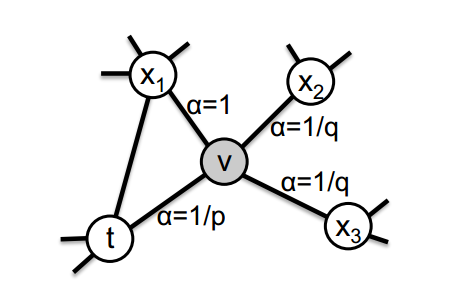
\includegraphics[width=0.5\textwidth]{figures/node2vec.png}
\end{center}
\caption{A random walk in the node2vec algorithm. The current node is the node
$v$ which was chosen as a neighbor to the vertex $t$.
Going back to $t$ is controlled by the parameter $p$, while going forward is
controlled by parameter $q$. The figure is copied from the original
paper~\cite{grover2016node2vec}.}
\label{node2vec_png}
\end{figure}

\subsubsection{LINE}

LINE (\cite{DBLP:journals/corr/TangQWZYM15}) is a network embedding model, able to handle very large, arbitrary types of graph networks $G=(V,E)$, (undirected, directed and/or weighted), by optimizing an objective which preserves both local and global network structures. Local structures are represented by the observed links in the networks, as for each pair of vertices linked by edge $(u, v)$, the weight $w_{uv}$ on that edge indicates the first-order proximity between u and v. Global structure is the second-order proximity between the vertices, determined through the shared neighborhood structures, as nodes with shared neighbors are likely to be similar. If $p_u = (w_{u,1}; \dots ;w_{u,|V|})$ denotes the first-order proximity of u with all the other vertices, then the second-order proximity between u and v is the similarity between $p_u$ and $p_v$.

In both cases, an objective function is defined and optimized, and the difference in the variants of the model that are described lies on whether first- or second-order proximity (or both) is used, and on the method selected for optimizing this objective in each case. Using first-order proximity, the KL-divergence between the joint and the empirical distribution of vertices $v_i$ and $v_j$ for each undirected edge $(i,j)$ is minimized. On the other hand, using second-order proximity, $u_i'$ is defined as the representation of $v_i$, when it is treated as a specific "context", and $u_i$ as the representation of $v_i$ when it is treated as a vertex. In this case, the KL-divergence between the conditional and the empirical distribution over the contexts is minimized.

A negative sampling approach tackles the problem of trivial infinity solutions in the case of first-order proximity and that of the computationally expensive minimization of the objective in the case of second-order proximity. Multiple negative edges are sampled according to some noisy distribution for each edge $(i,j)$, and asynchronous Stochastic Gradient Descent algorithm is used, which, in each step, samples a mini-batch of edges and updates the model parameters.
When edge weights have a high variance, scales of the gradients in SGD diverge, making it harder to find a good learning rate. Optimization via edge-sampling is then applied, by sampling from the original edges, with sampling probabilities proportional to the original edge weights. Sampled edges are treated as binary edges.

To combine first- and second-order proximity, a simple way is to concatenate the vector representations learned by both into a longer vector, and reweigh the dimensions, to balance the two representations. It was found that in practice, optimization takes $O(|E|)$ time, and the overall complexity of LINE is $O(d(K+1))$, given that K is the number of negative samples and $d<<|V|$ the dimension of the lower-dimensional space.

As a way to better combine first- and second-order proximities, the authors propose to jointly train the objective function in the future. Also, they suggest that higher-order proximity approaches could be applied to provide a better result. Another objective could be to find new embeddings of heterogeneous information networks, meaning graphs with vertices of multiple types. Furthermore, the case of no observed connections between new and existing vertices could be explored in the future by resorting to other network information, such as the textual information of the vertices.

\subsubsection{HARP}

HARP (\cite{DBLP:journals/corr/ChenPHS17}) is a meta strategy which solves the graph representation learning problem using a hierarchical approach.
All methods described before could easily get stuck at a bad local minima as the result of poor initialization of the non-convex optimization. Moreover,these methods mostly aim to preserve local proximities in a graph but neglect its global structure.

HARP recursively coalesces the nodes and edges in the original graph to get a series of successively smaller but structurally similar graphs . These coalesced graphs, each with a different granularity, provide a view of the original graph’s global structure. Starting from the most simplified form, each graph is used to learn a set of initial representations which serve as good initializations for embedding the next, more detailed graph. This process is repeated until we get an embedding for each node in the original graph.

HARP's method for multi-level graph representation learning consists of three parts:
\begin{itemize}
    \item \textbf{Graph Coarsening:} starting from the original graph, $G = G_0$, a hierarchy of successively smaller graphs $G_0, G_1, \dots , G_L$ is created. A hybrid graph coarsening scheme is developed, which is repeatedly applied to obtain a small graph. It combines two algorithms, edge collapsing and star collapsing, preserving first- and second-order proximity respectively. Edge collapsing is an edge selection and node merging algorithm, which arbitrarily merges nodes of edges into single nodes, providing a graph with at least half the edges of the original one. Star collapsing algorithm, on the other hand, considers star-like structured graphs, and merges nodes with the same neighbors into supernodes.
    \item \textbf{Graph Embedding:}  Using a provided Graph Embedding algorithm, Graph Embedding is obtained on the Coarsest Graph $G_L$, a small sized graph providing a high quality representation.
    \item \textbf{Representation Prolongation and Refinement:} For each graph $G_i$, the graph representation of $G_{i+1}$ is prolonged and taken as its initial embedding, $\Phi'_{G_i}$, followed by applying a provided embedding algorithm to $(G_i, \Phi'_{G_i})$ to further refine $\Phi'_{G_i}$ and obtain refined embedding $\Phi_{G_i}$.
\end{itemize}

Processes of Graph Embedding, Prolongation and Refinement are then applied recursively to the larger graphs and their embeddings, until we obtain the graph embedding of the original graph, $\Phi'_{G_0}$.

HARP is combined with a few state-of-the-art graph embedding methods (DeepWalk, LINE, Node2vec) to produce higher quality embeddings for all of them.
Time Complexity of HARP(DW) is the same as that of the original DeepWalk, equal to $O(\gamma |V|tw (d+dlog|V|))$, where $\gamma$ is the number of random walks, t is the  walk length, w is the window size, d is the representation size, and $|V|$ is the number of nodes. Similarly, time complexity of HARP(LINE) is the same as that of LINE, $O(r|E|)$,  linear to the number of edges in the graph, $|E|$, and the number of iterations over edges, r.


\section{Graph Convolutional Networks}

The recent popularity of convolutional neural networks \cite{40k}, and their
success in classifying images and other tasks with a striking accuracy, has intrigued the scientific
community with the question of whether -at least a variant of them- can be leveraged in learning tasks
of graph networked data. The use of graph structures in computer
vision\cite{survey}, as well in the representation of social networks
\cite{kleinberg_book}, has made this task look appealing and worth of investigation-research.
However, using convolutional neural networks for
networked data directly, is not straightforward and it poses significant
challenges.\\
\spara{Challenges in Graph Convolutional Networks} First and foremost,
as CNNs were mainly used for image classification, they assume that
data lie on a regular grid in a geometric space (most commonly
Euclidean). On the contrary, graph data are a typical form of unordered data that lie in
an irregular domain. Also, the heavy-tailed distribution of node degrees
in real networks \cite{smth} makes the filtering-convolution part difficult,
as it is not easy to define a constant-sized neighborhood and apply a
localized filter, as in the traditional CNN case. Also, the pooling stage has to
be defined as well.
\spara{Convolution in graphs} First efforts to address the above mentioned issues
by Bruna et al. \cite{Lecun} and introduce the architecture of CNNs to networked data,
mainly draw from the field of Graph Signal Processing \cite{shuman}.
Graphs are generally considered undirected and their representation is given
through their \textbf{Laplacian $L = D -A$} or more commonly the normalized
\textbf{Laplacian $L = I_n - D^{-\frac{1}{2}}AD^{-\frac{1}{2}}$}. As this matrix
is a real symmetric and positive semidefinite, it admits an eigenvector
decomposition $L=U\Lambda U^T$, where $U$ is a square orthonormal matrix with
the eigenvectors as its columns, and $\Lambda$ is the diagonal matrix of eigenvalues.
Letting $x\in \mathbb{R}^{n}$ be a feature vector of the nodes of a graph,
the {\em graph fourier transform} is then defined as $\hat{x}=U^T x \in \mathbb{R}^n$
and its inverse as $x = U\hat{x}$. The \textbf{convolution operator} on a graph
$\mathcal{G}$ is defined on the Fourier domain, as:
\begin{equation*}
x *_{\mathcal{G}} y = U((U^T x)\odot (U^T y))
\end{equation*}
where $\odot$ denotes the element-wise Hadamard product.\\
Therefore, a signal $x$ is filtered by $g_{\theta}$, as:\\
\begin{equation}
y = g_{\theta}(L)x = g_{\theta} (U\Lambda U^T)x = U g_{\theta}(\Lambda ) U^T x
\end{equation}
where $g_{\theta}(\Lambda) = diag(\theta)$ is a non-parametric filter.\\
This approach has, however, the following limitations:
\begin{itemize}
\item [1.] Filters are not localized
\item [2.] Their learning complexity scales with the dimensionality of the data $O(n)$
\item [3.] The computational cost of filtering is high- $O(n^2)$, due to the
multiplication with the Fourier basis $U$.
\end{itemize}

\subsubsection*{ChebNet\cite{defferard}}
Deferrard et al. \cite{defferard} were the first to propose a way to deal with
the above issues.\\
\spara{Localized Filter} First of all, they propose the use of a polynomial filter:\\
\begin{equation}
g_{\theta}(\Lambda ) = \sum_{k=0}^{K-1}\theta_k \Lambda^k
\end{equation}
where the parameter $\theta \in \mathbb{R}^K$ is a vector of polynomial
coefficients. As $(L^K)_{i,j} = 0$ whenever $d_{\mathcal{G}}(i,j)>K$, these
spectral filters are $K$-localized.\\
\spara{Learning complexity} Their learning complexity is equal to the support
size of the filter, hence $O(K)$, as in conventional CNNs.\\
\spara{Computational cost of filtering} As mentioned earlier, because of the
multiplication of the filter with the Fourier basis $U$, the computational cost
is relatively high, $O(n^2)$. For this reason, the express the filter as a
Chebyshev polynomial of order $k$, that can be computed using the recurrence
$T_k(x) = 2xT_{k-1}(x)-T_{k-2}(x)$ with $T_o = 1$ and $T_1 = x$. Thus, the whole
filtering operation can be written as $y = g_{\theta}(L)x =
\sum_{k=0}^{K-1}\theta_k T_k (\widetilde{\Lambda })x$, where $T_k (\Lambda ) \in
\mathbb{R}^{nxn}$ is the Chebyshev polynomial of order $k$ evaluated at the
scaled Laplacian $\widetilde{\Lambda} = 2L/\lambda_{max} - I_n$, using the
recurrence $\bar{x}_k = 2\widetilde{\Lambda}\bar{x}_{k-1} - \bar{x}_{k-2}$, with
$\bar{x}_0 = x$ and $\bar{x}_1 = \widetilde{\Lambda}x$. The cost of the
filtering operation becomes then $O(K|E|)$, as it is a multiplication of a
sparse matrix with a column vector of size $K$.\\
\spara{Graph Coarsening and Pooling}
Pooling on traditional convolutional neural networks, is performed usually on a
patch of neighboring pixels on an image. However, in graphs, we can not explicitly
define this notion of neighborhood as in a Euclidean grid. Therefore, the authors of
this paper propose a multilevel clustering approach, that not only clusters
similar vertices - in a topological fashion- together, but also produces coarser
versions of the graph on each level, resembling closely the pooling operation of traditional
CNNs. The multilevel clustering algorithm chosen is Graclus \cite{Kulis}.\\
In order to perform pooling in a fast and memory efficient manner, nodes are
organized in a balanced binary tree. Specifically, after coarsening, each node
has either two childer, if it was matched at the finer level, or one, if it was
not. Those singleton nodes are paired with fake nodes, having a neutral value
-with respect to the activation function- as its input. On the following figure,
we can see a visualization of this pooling procedure:\\

its input signal.
\subsubsection*{Kipf}

\subsubsection*{GraphSAGE}

\section{Comparative Evaluation}

\subsection{Datasets}

The world is full of graphs and this shows in the available datasets. From citation networks to
online communities to biological networks, all are available online.  We focused on five datasets
for the matrix factorization and random walk based algorithms.

For each dataset we have kept only the largest weakly connected component, as network embeddings
have no meaning between disconnected components.

{\bf \href{https://snap.stanford.edu/data/email-Eu-core.html}{email-EU-core}}: This dataset was
generated using email data from a large European research institution. There is an edge between
nodes $u$ and $v$ if person $u$ sent an email to person $v$.  Each person belongs to one of the 42
departments of the institution. The dataset contains 986 nodes and 25552 edges.

{\bf \href{https://snap.stanford.edu/data/com-Youtube.html}{com-Youtube}~\cite{mislove-2007-socialnetworks}}:
This is the largest dataset we used with 1134890 nodes and 2987624 edges. Edges are friendships and
the classes are user defined groups.

{\bf \href{https://snap.stanford.edu/data/com-DBLP.html}{dblp}}: This is a citation network from
computer science research papers. Every author is a node and two authors are connected if they have
co-authored one paper. Each community is a publication venue where the authors published. The
network has 317080 nodes and 1049866 edges.

{\bf \href{https://snap.stanford.edu/data/com-Amazon.html}{com-amazon}}: This dataset was collected
by crawling the Amazon website. Each node is a product and two products are connected if they appear
in Amazon's {\it Customers Who Bought This Item Also Bought} feature. The groundtruth communities
are the connected components in each product category.  This network has 334863 nodes and 925872
edges.

{\bf \href{http://snap.stanford.edu/graphsage/}{PPI}~\cite{hamilton2017inductive}}: Protein-Protein
Interaction network. Each node in this network corresponds to a protein and and edge exists between
two proteins if an interaction between them has been recorded. There are 24 disconnected graphs
correcsponding to different human tissues.  The labels come from gene ontology (121)
from~\cite{subramanian2005gene}. The average graph has 2360 nodes and average degree 14.4.

{\bf \href{https://github.com/tkipf/gcn/tree/master/gcn/data}{Citeseer, Pubmed, Cora}~\cite{kipf2016semi}}: We also consider three citation network datasets: Citeseer, Cora and Pubmed (Sen et al., 2008). The datasets contain sparse bag-of-words feature vectors for each document and a list of citation links between documents. We treat the citation links as (undirected) edges and construct a binary, symmetric adjacency matrix A. Each document has a class label. For training, we only use 20 labels per class, but all feature vectors.

\subsection{Evaluation Tasks}

\subsection{Comparative Evaluation}

Unfortunately not all algorithms could be run on all the datasets. MDS and Spectral Embedding
require quadratic space with respect to the number of the nodes, giving them an effective ceiling of
about 10000 nodes. The largest dataset, com-Youtube proved too much for all implementations except
deepwalk. We were unable to run the published code for LINE, depsite our best efforts.

The following table~\ref{tab:results} shows the micro and macro precision, recall and F1 score for
classification in each dataset.

\begin{table}[h]
    \captionof{table}{Classification results on different embedding algorithms and datasets}\label{tab:results}
\centerline{
\begin{tabular}{ll|rrr|rrr|r}
\toprule
    &                   &  \multicolumn{3}{c|}{micro} &  \multicolumn{3}{c|}{macro} & weighted \\
    &                   &  Precision & Recall & F1 &  Precision &  Recall &  F1 &  F1 \\
\midrule
\multirow{5}{*}{email-EU-core} & deepwalk & \cellcolor{yellow!75} 0.9550 & \cellcolor{yellow!75} 0.9550 & \cellcolor{yellow!75} 0.9550 & \cellcolor{yellow!75} 0.9181 & \cellcolor{yellow!75} 0.9264 & \cellcolor{yellow!75} 0.9144 & \cellcolor{yellow!75} 0.9482 \\
 & node2vec & 0.6113 & 0.6113 & 0.6113 & 0.3065 & 0.3561 & 0.3035 & 0.5507 \\
 & HARP & 0.6923 & 0.6923 & 0.6923 & 0.5181 & 0.5296 & 0.4901 & 0.6535 \\
 & MDS & 0.0324 & 0.0324 & 0.0324 & 0.0454 & 0.0441 & 0.0278 & 0.0291 \\
 & SpectralEmbedding & 0.6640 & 0.6640 & 0.6640 & 0.5976 & 0.5797 & 0.5467 & 0.6706 \\
\cline{1-9}
com-Youtube & deepwalk & 0.9029 & 0.9029 & 0.9029 & 0.5650 & 0.9117 & 0.5674 & 0.9426 \\
\cline{1-9}
\multirow{3}{*}{dblp} & deepwalk & 0.9457 & 0.9457 & 0.9457 & 0.6299 & 0.8954 & 0.6683 & 0.9610 \\
 & node2vec & 0.9557 & 0.9557 & 0.9557 & 0.6373 & \cellcolor{yellow!75} 0.9376 & 0.6879 & 0.9677 \\
 & HARP & \cellcolor{yellow!75} 0.9565 & \cellcolor{yellow!75} 0.9565 & \cellcolor{yellow!75} 0.9565 & \cellcolor{yellow!75} 0.6521 & 0.9040 & \cellcolor{yellow!75} 0.6964 & \cellcolor{yellow!75} 0.9679 \\
\cline{1-9}
\multirow{3}{*}{com-amazon} & deepwalk & 0.9985 & 0.9985 & 0.9985 & \cellcolor{yellow!75} 0.9829 & 0.9854 & 0.9828 & 0.9985 \\
 & node2vec & 0.9980 & 0.9980 & 0.9980 & 0.9615 & \cellcolor{yellow!75} 0.9944 & 0.9750 & 0.9981 \\
 & HARP & \cellcolor{yellow!75} 0.9987 & \cellcolor{yellow!75} 0.9987 & \cellcolor{yellow!75} 0.9987 & 0.9814 & 0.9913 & \cellcolor{yellow!75} 0.9847 & \cellcolor{yellow!75} 0.9987 \\
\cline{1-9}
\multirow{5}{*}{PPI} & deepwalk & 0.6617 & 0.6617 & 0.6617 & 0.6088 & 0.6409 & 0.6060 & 0.6821 \\
 & node2vec & 0.6540 & 0.6540 & 0.6540 & 0.6079 & 0.6410 & 0.6022 & 0.6761 \\
 & HARP & 0.6610 & 0.6610 & 0.6610 & 0.6100 & \cellcolor{yellow!75}0.6427 & 0.6064 & 0.6819 \\
 & MDS & 0.5294 & 0.5294 & 0.5294 & 0.5005 & 0.5009 & 0.4770 & 0.5621 \\
 & SpectralEmbedding & \cellcolor{yellow!75} 0.6911 & \cellcolor{yellow!75} 0.6911 & \cellcolor{yellow!75} 0.6911 & \cellcolor{yellow!75} 0.6178 & 0.6419 & \cellcolor{yellow!75} 0.6211 & \cellcolor{yellow!75} 0.7040 \\
\bottomrule
\end{tabular}
}
\end{table}


The only method that lags behind every other algorithm by a lot. Deepwalk remains always very close
to the best algorithm. In email-EU-core all algorithms other than deepwalk perform horribly
comparably. HARP which utilizes deepwalk has the best performance in the dblp dataset. It is
surprising that while Spectral Embedding is so old, in the PPI dataset outperforms all other
methods. The authors believe that this is because the PPI graphs have very small cuts that
correspond to the the cuts between clusters of interacting proteins.

As stated at the start of this report, no single algorithm can produce embeddings superior to all
others for all algorithms. Even a single algorithm is usually highly customizable with many
parameter choices whose optimums change depending on the input graph.



Table \ref{table:1} is \dots
\begin{table}[h!]
\centering
\caption{Prediction results for PPI dataset (micro-averaged F1 scores). \newline}
\begin{tabular}{|p{3cm}||p{3cm}|p{3cm}|}
 \hline
 \multicolumn{3}{|c|}{\textbf{PPI}} \\
 \hline
 & Supervised F1 &Unsupervised F1\\
 \hline\hline
 DeepWalk   & ---    &0.39\\
 max\_pool &   0.45131  & \textbf{0.47} \\
 mean\_pool &\textbf{0.51893} & 0.45\\
 GCN    &0.45438 & 0.44\\
 \hline
\end{tabular}\\
\label{table:1}
\end{table}

Table \ref{table:2} is \dots
\begin{table}[h!]
\centering
\caption{}
\begin{tabular}{ |p{2cm}||p{2cm}|p{2cm}|p{2cm}|p{2cm}|p{2cm}|}
 \hline
 &\multicolumn{3}{c}{\textbf{Order of Chebyshev's Polynomial}} &&\\
 \hline
 &K=1& K=2 &K=3 &GCN & GraphSAGE\\
 \hline\hline
 Cora   & 0.7990    &0.84362 &0.793 &0.809 &\textbf{0.849}\\
 citeseer &   0.702  & 0.692 &0.68 &\textbf{0.715}& --- \\
 pubmed &0.71480 & 0.713 &0.74 &0.792 &\textbf{0.837}\\
 \hline
\end{tabular}\\
\label{table:2}
\end{table}



\section{Conclusion}




\bibliography{iclr2019_conference}
\bibliographystyle{iclr2019_conference}

\end{document}
